\section{Introduction}

Humans use different forms of communications such as speech, hand gestures and emotions. Being able to understand one's emotions and the encoded feelings is an important factor for an appropriate and correct understanding.


With the ongoing research in the field of robotics, especially in the field of humanoid robots, it becomes interesting to integrate these capabilities into machines allowing for a more diverse and natural way of communication. One example is the Software called EmotiChat~\cite{Anderson06areal-time}. This is a chat application with emotion recognition. The user is monitored and whenever an emotion is detected (smile, etc.), an emoticon is inserted into the chat window. Besides Human Computer Interaction other fields like surveillance or driver safety could also profit from it. Being able to detect the mood of the driver could help to detect the level of attention, so that automatic systems can adapt.\\
\let\thefootnote\relax\footnote{*F. Trier and P. Burkert contributed equally to this work.}


Many methods rely on extraction of the facial region. This can be realized through manual inference~\cite{4032815} or an automatic detection approach~\cite{Anderson06areal-time}.
Methods often involve the Facial Action Coding System (FACS) which describes the facial expression using Action Units (AU). An Action Unit is a facial action like "raising the Inner Brow". Multiple activations of AUs describe the facial expression~\cite{kumar2009face}. Being able to correctly detect AUs is a helpful step, since it allows making a statement about the activation level of the corresponding emotion. \\
Handcrafted facial landmarks can be used such as done by Kotsia et al.~\cite{4032815}. Detecting such landmarks can be hard, as the distance between them differs depending on the person~\cite{6998925}. Not only AUs can be used to detect emotions, but also texture. When a face shows an emotion the structure changes and different filters can be applied to detect this~\cite{6998925}.\\


\begin{figure}
   \centering
        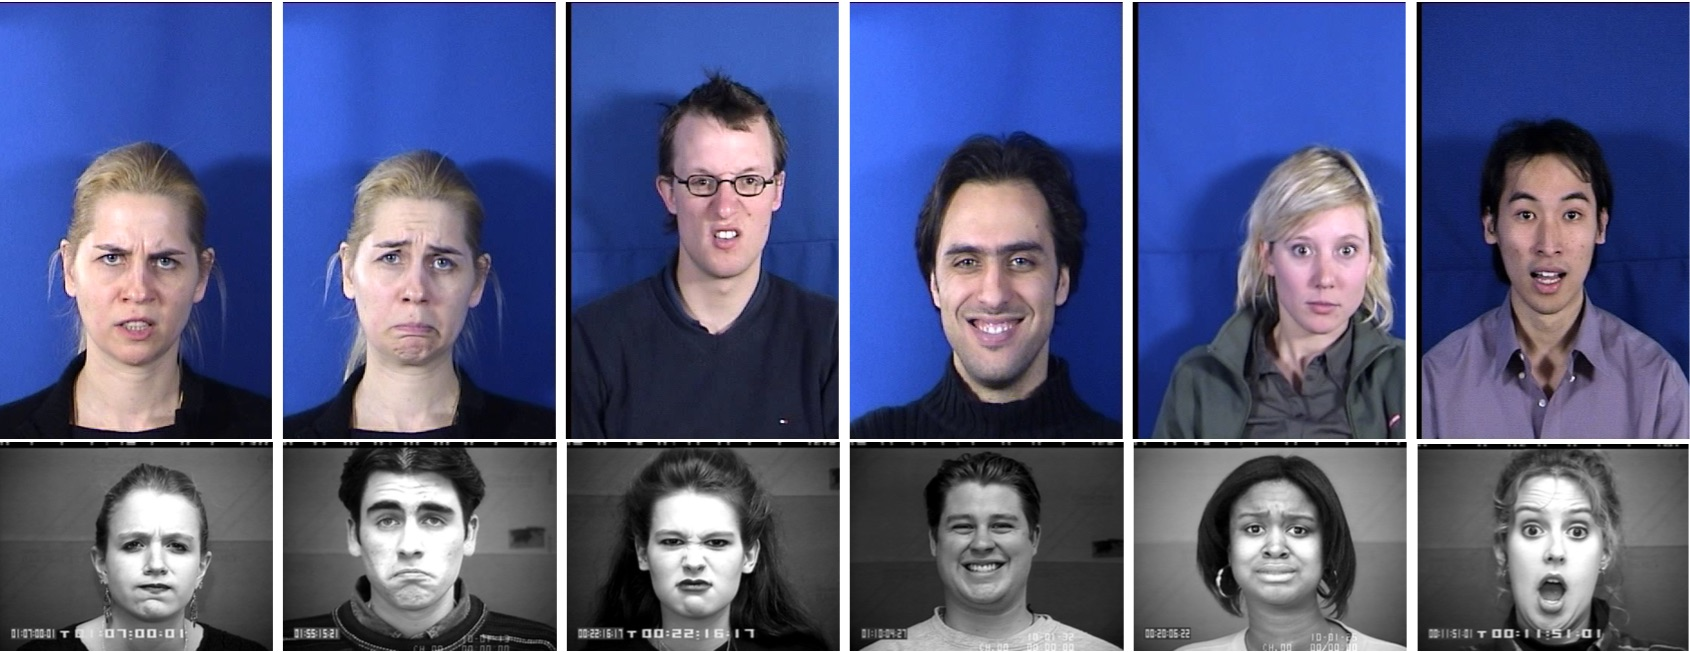
\includegraphics[width=\columnwidth]{Fig1}
   \caption{Example images from the MMI (top) and CKP (bottom). The emotions from left to right are: \textit{Anger}, \textit{Sadness}, \textit{Disgust}, \textit{Happiness}, \textit{Fear}, \textit{Surprise}. The emotion \textit{Contempt} of the CKP set is not displayed.}\label{fig:example_images}
\end{figure}




The presented approach uses Artificial Neural Networks (ANN). ANNs differ, as they are trained on the data with less need for manual interference. 
Convolutional Neural Networks are a special kind of ANN and have been shown to work well as feature extractor when using images as input~\cite{donahue2013decaf} and are real-time capable. This allows for the usage of the raw input images without any pre- or postprocessing.\\
GoogleNet~\cite{DBLP:journals/corr/SzegedyLJSRAEVR14} is a deep neural network architecture that relies on CNNs. It has been introduced during the Image Net Large Scale Visual Recognition Challenge(ILSVRC) 2014. This challenge analyses the quality of different image classification approaches submitted by different groups. The images are separated into 1000 different classes organized by the WordNet hierarchy. In the challenge "object detection with additional training data" GoogleNet has achieved about 44\% precision~\cite{LSVRC-results}. These results have demonstrated the potential which lies in this kind of architecture. Therefore it has been used as inspiration for the proposed architecture.\\
The proposed network has been evaluated on the Extended Cohn-Kanade Dataset (Section~\ref{sec:ckp}) and on the MMI Dataset (Section~\ref{sec:mmi}). Typical pictures of persons showing emotions can be seen in Fig.~\ref{fig:example_images}.
The emotion \textit{Contempt} of the CKP set is not shown as no subject with consent for publication and an annotated emotion is part of the dataset. Results of experiments on these datasets demonstrate the success of using a deep layered neural network structure. With a 10-fold cross-validation a recognition accuracy of 99.6\% has been achieved. \\

The paper is arranged as follows: After this introduction, Related Work (Section~\ref{sec:related}) is presented which focuses on Emotion/Expression recognition and the various approaches scientists have taken. Next is Section~\ref{sec:background}, Background, which focuses on the main components of the architecture proposed in this article. Section~\ref{sec:datasets} contains a summary of the used Datasets. In Section~\ref{sec:architecture} the architecture is presented. This is followed by the experiments and its results (Section~\ref{sec:experiments}) . Finally, Section~\ref{sec:conclusion} summarizes the article and concludes the article.